%\documentclass[12pt]{article}
\documentclass[12pt, twocolumn]{article}
\usepackage{siunitx}
\usepackage[style=authoryear, backref]{biblatex}
\usepackage{listings}
\usepackage{graphicx}
\usepackage[hidelinks]{hyperref}
\usepackage{amsmath, wasysym}
\usepackage{microtype}
\usepackage[all]{nowidow}
\hypersetup{frenchlinks=true}
\addbibresource{references.bib}
\newcommand*\aap{A\&A}
\let\astap=\aap
\newcommand*\aapr{A\&A~Rev.}
\newcommand*\aaps{A\&AS}
\newcommand*\actaa{Acta Astron.}
\newcommand*\aj{AJ}
\newcommand*\ao{Appl.~Opt.}
\let\applopt\ao
\newcommand*\apj{ApJ}
\newcommand*\apjl{ApJ}
\let\apjlett\apjl
\newcommand*\apjs{ApJS}
\let\apjsupp\apjs
\newcommand*\aplett{Astrophys.~Lett.}
\newcommand*\apspr{Astrophys.~Space~Phys.~Res.}
\newcommand*\apss{Ap\&SS}
\newcommand*\araa{ARA\&A}
\newcommand*\azh{AZh}
\newcommand*\baas{BAAS}
\newcommand*\bac{Bull. astr. Inst. Czechosl.}
\newcommand*\bain{Bull.~Astron.~Inst.~Netherlands}
\newcommand*\caa{Chinese Astron. Astrophys.}
\newcommand*\cjaa{Chinese J. Astron. Astrophys.}
\newcommand*\fcp{Fund.~Cosmic~Phys.}
\newcommand*\gca{Geochim.~Cosmochim.~Acta}
\newcommand*\grl{Geophys.~Res.~Lett.}
\newcommand*\iaucirc{IAU~Circ.}
\newcommand*\icarus{Icarus}
\newcommand*\jcap{J. Cosmology Astropart. Phys.}
\newcommand*\jcp{J.~Chem.~Phys.}
\newcommand*\jgr{J.~Geophys.~Res.}
\newcommand*\jqsrt{J.~Quant.~Spec.~Radiat.~Transf.}
\newcommand*\jrasc{JRASC}
\newcommand*\memras{MmRAS}
\newcommand*\memsai{Mem.~Soc.~Astron.~Italiana}
\newcommand*\mnras{MNRAS}
\newcommand*\na{New A}
\newcommand*\nar{New A Rev.}
\newcommand*\nat{Nature}
\newcommand*\nphysa{Nucl.~Phys.~A}
\newcommand*\pasa{PASA}
\newcommand*\pasj{PASJ}
\newcommand*\pasp{PASP}
\newcommand*\physrep{Phys.~Rep.}
\newcommand*\physscr{Phys.~Scr}
\newcommand*\planss{Planet.~Space~Sci.}
\newcommand*\pra{Phys.~Rev.~A}
\newcommand*\prb{Phys.~Rev.~B}
\newcommand*\prc{Phys.~Rev.~C}
\newcommand*\prd{Phys.~Rev.~D}
\newcommand*\pre{Phys.~Rev.~E}
\newcommand*\prl{Phys.~Rev.~Lett.}
\newcommand*\procspie{Proc.~SPIE}
\newcommand*\qjras{QJRAS}
\newcommand*\rmxaa{Rev. Mexicana Astron. Astrofis.}
\newcommand*\skytel{S\&T}
\newcommand*\solphys{Sol.~Phys.}
\newcommand*\sovast{Soviet~Ast.}
\newcommand*\ssr{Space~Sci.~Rev.}
\newcommand*\zap{ZAp}

\title{Simulating the influence of Stellar Winds and Supernovae in Open Clusters} \author{R.\,S.~Dullaart \and R.\,J.\,R.~Rijnenberg \and W.\,W.\,M.~van~Tol} \date{\today}

\begin{document}
\twocolumn[
\begin{@twocolumnfalse}
    \maketitle
    \begin{abstract}
    %\textcolor{red}{
    \footnotesize     
    Many open clusters disband after formation partly due to gas expulsion. The aim of this project is to find out whether stellar winds or supernovae are a bigger cause of gas expulsion in open clusters. With AMUSE we can simulate the interactions between stars and gas in a cluster by bridging hydrodynamic code with gravitational code and adding stellar evolution code to drive stellar winds and create a supernova.
    When running initial simulations we do not get interactions between wind and gas. After adjusting the code we run a smaller simulation which shows a small increase in velocity and kinetic energy of the original gas of the cluster and a small decrease in density of the cluster. This shows that the code works, but there are a few small flaws left in the code. The simulated effect of winds is too small to give a concise answer to the research question.
    %}
    \end{abstract}
\end{@twocolumnfalse}]

% \section*{Requirements}
% {\footnotesize\begin{enumerate}
%     \item Introduction with a motivation for the selected topic
%     \item Methods
%     \begin{enumerate}
%         \item Creativity: Stick to known methods to Develop novel method
%         \item Valid approach: You miss vital aspects of the problem or You cover all vital aspects of the problem
%         \item Assumptions with motivation for the various ingredients and their coupling (should include a flow-chart and doodle of the astrophysical setup)
%         \item Choice of model parameters and initial conditions (with a doodle of the parameter space)
%     \end{enumerate}
%     \item Results (at least two figures showing results)
%     \begin{enumerate}
%         \item It is difficult to impossible to interpret your results or Your results are easily interpreted
%     \end{enumerate}
%     \item Discussion (should contain a discussion on the caveats and future prospects)
%     \begin{enumerate}
%         \item Numerical effects: You do not critically evaluate numerical effects or You clearly state what numerical effects impact your results
%         \item Validity of conclusions: Your conclusions are not supported by your results or Your results conclusively demonstrate your results
%     \end{enumerate}
%     \item Conclusions (if any)
% \end{enumerate}}
% \newpage

\section{Introduction}
The present day accepted theory on star formation is that most stars are born in groups \parencite{lada2003}, also known as star clusters.
While some of these clusters stay grouped together for up to 100 -- \SI{1000}{\mega yr}, some clusters dissolve into their host galaxy within a few \si{\mega yr}.
While open clusters themselves have been the subject of many observations, the mechanism behind the boundedness of these clusters is still not well known.

Open clusters are groups of about 100 to \num{10000} stars which are loosely bound by gravity.
An open cluster forms stars from the same gas cloud and it's formation period is small enough compared to it's lifetime, that we can consider the ages, positions and composition of all stars in the cluster as approximately the same \parencite{Open_star_clusters}.
Since the masses of the stars are different, the evolutionary stage of the cluster can be accurately determined.
This means we can have a good idea of the shape of the Hertzsprung-Russel diagram (HRD) of open clusters and therefore accurately determine their metallicity and age using isochrones \parencite{girardi2002}.
Apart from that, the HRDs can be used to obtain a measure for the gas extinction between the cluster and the observer.
All in all they can be used to determine the structure of the Milky Way Galaxy.

A problem with these measurements is that not all stars that form together end up in a cluster.
We know for instance that many open clusters disband after formation and dissolve in the host galaxy.
In other words the criteria for the boundedness are still a case for study.
One of the reasons a cluster dissolves into the host galaxy is that the stars in the cluster are blown away with the left over gas that was not used up in the star formation.
Therefore the structure of the Milky Way constructed using open clusters is biased by the formation conditions of actually forming an open cluster.

In this work we are going to look at the processes that remove the excess gas in open clusters.
There are two factors that blow this gas away.
Firstly, there is the stellar wind consisting of blown away particles from the star, which can blow the interstellar medium away.
The second mechanism are the powerful blasts from supernovae.
After supernovae have exploded, most of the gas from the cluster is removed, but it's unknown how much gas was still present just before the first stars in the cluster enter the supernova stage.
Therefore we'll investigate whether stellar winds or supernova explosions are the primary factor for gas expulsion in open clusters.


\section{Methods}
In order to test the boundedness of open clusters, we'll create a simulation a newly formed star cluster.
In order to create this simulated cluster, we use The Astrophysical Multipurpose Software Environment (AMUSE) to model the kinematics of the gas and stars and the evolution of our system \parencite{AMUSE_book, AMUSE1, AMUSE2, AMUSE3}.
The simulation will combine the positions and velocities of stars and gas particles and includes N-body gravitational interactions between the stars and hydrodynamic interactions between the gas particles.
Furthermore we use a model for stellar evolution and the generation of stellar winds to create a detailed simulation of the cluster.

In this section, we'll first describe in Sec. \ref{sec:m:init} what initial conditions we use to generate a cluster. Section \ref{sec:m:star-evo} goes into detail about why and how we implement the evolution of the cluster members. The last part, Sec. \ref{sec:m:bridging}, will describe the interactions between the different codes and their different timesteps.

\subsection{Initial conditions}\label{sec:m:init}
We assume that clusters start their life as being stable systems which could lose their stability by small perturbations during their lifetime.
Therefore we start by creating a stable system of stars and gas.
The system should not be virialised, because then the system will too stable, while a real open cluster is only loosely bound by gravity.
We therefore need a system where not only the interaction between the gas, but also between the stars can become unstable when small perturbations are added.

\begin{figure*}[ht]
    \centering
    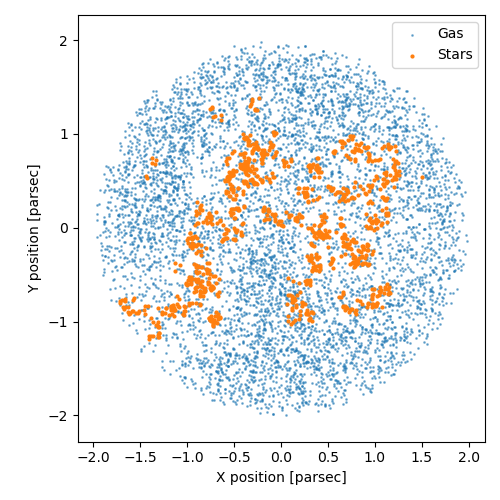
\includegraphics[width=0.6\linewidth]{figures/initial_position.png}
    \caption{An example of a simulated cluster using a fractal distribution for the stars (orange) and a molecular cloud distribution for the gas (blue). Some of the gas around the stars has been removed to simulate stars being created from the initial cloud.}
    \label{fig:m:fractal-cluster}
\end{figure*}

The theory of star formation states that star formation starts when a gas cloud becomes smaller than the Jeans length $\lambda_{\text{J}}$, given by
\begin{equation}
    \lambda_{\text{J}}=\left({\frac {15k_{\text{B}}T}{4\pi Gm_{p}\mu \rho }}\right)^{\frac {1}{2}},
\end{equation}
where $k_\text{B}$ is Boltzmann's constant, $T$ the temperature of the cloud, $G$ Newtons gravitational constant, $m_p$ the proton mass, $\mu$ the mean molecular weight of the gas and $\rho$ the density of the gas cloud.
When the cloud reaches the Jeans length, it starts to collapse.
Due to the increase in density, parts within the collapsing cloud now also get smaller than the Jeans length and sub parts of the cloud start collapsing into themselves.
In the end the initial cloud will have formed multiple stars close together.

To mimic this behaviour in our simulation, we use a fractal cluster model \parencite{AMUSE-FractalCluster} to initialise the stars' positions.
This model starts with defining a cubic space called the parent cube in which the fractal cluster will be formed.
This cube is divided in $N_{\text{div}}^3$ subcubes or children, which have a $N_{\text{div}}^{3-D}$ probability to become a new parent cube, where $D$ is the fractal dimension.
This process of subdivision is then repeated for the new parent cubes until there are as many new parent cubes as the wanted number of stars.
One example fractal distribution is displayed in orange in Fig. \ref{fig:m:fractal-cluster}.
For the simulations we use a division parameter of $N_\text{div}=2$ and a fractal dimension of $D=1.6$ to create a cluster containing $n_{\text{stars}} = 100$ stars with a cluster radius of \SI{1}{pc}.

The initial masses of the stars follow a Salpeter distribution \parencite{salpeter}, given by
\begin{equation}
    \xi (m)\Delta m=\xi _{0}\left({\frac {m}{M_{\odot }}}\right)^{-\alpha}\left({\frac {\Delta m}{M_{\odot }}}\right).
\end{equation}
Here $\xi_0$ is a constant and the exponent $\alpha = 2.35$.
We use a scaled version of this distribution to get 1000 masses between 0.1 and \SI{100}{M_{\astrosun}}.

The gas will be simulated using smoothed particle hydrodynamics (SPH) codes.
We used the SPH code \texttt{Fi} \autocite{AMUSE-Fi1, AMUSE-Fi2, AMUSE-Fi3, AMUSE-Fi4} to simulate the hydrodynamics of the gas which will be pushed away by the supernova and the radiation from the stars.
We chose an SPH code above a grid based code since we want to have infinite range for the gas to be blown away to.
As initial conditions we will assume a molecular cloud distribution for the positions and velocities of the gas.
This distribution creates $N$ particles of equal mass in a homogeneous sphere, but with a turbulent velocity distribution \parencite{AMUSE_book, AMUSE-molecular-cloud}.
Using a predefined star-to-gas-mass ratio, the gas mass is determined and a gas cloud containing the combined mass of the stars and the wanted gas mass is created.
From this molecular gas sphere, for each star the gas closest to it is removed up to the star's mass.
That way, the gas distribution contains holes where stars were formed and since the mass of the stars was removed from the distribution, the resulting mass complies to the star-to-gas-mass ratio.
The observed average star formation efficiency (SFE), 
\begin{equation}
\epsilon = \frac{M_{\text{stars}}}{M_{\text{stars}}+M_{\text{gas}}},
\end{equation}
over the lifetime of a cluster lies between 0.05 and 0.5 \parencite{star-formation-efficiency}.
For this simulation, we used $N=\num{10000}$ gas particles and a star-to-gas-mass ratio of $0.2$, which results in a SFE of $\epsilon \approx 0.16$.
An example of the resulting cluster where the gas around the stars has been removed can be found in Fig. \ref{fig:m:fractal-cluster}.

For the gravitational dynamics of the stars we use the direct N-body integrator \texttt{ph4} \parencite{AMUSE_book}, which is a block time step fourth-order Hermite direct N-body code.
In other words, this code solves Newton's equations of motion without free physical parameters.
The only tunable parameter is the timestep.


\subsection{Stellar evolution}\label{sec:m:star-evo}
There are two important factors which can disrupt the initial stable system and therefore unbound a part of the cluster.
The first one is a supernova explosion that is presumably the biggest cause of gas expulsion from the cluster.
In general a supernova explosion blows away all the free gas in a cluster.
This means that it's necessary to simulate the evolution of the stars in our cluster to simulate a supernova. 
We use the stellar evolution code SeBa \parencite{AMUSE-SeBa1, AMUSE-SeBa2} to let the stars evolve over time.

\begin{figure*}[ht]
    \centering
    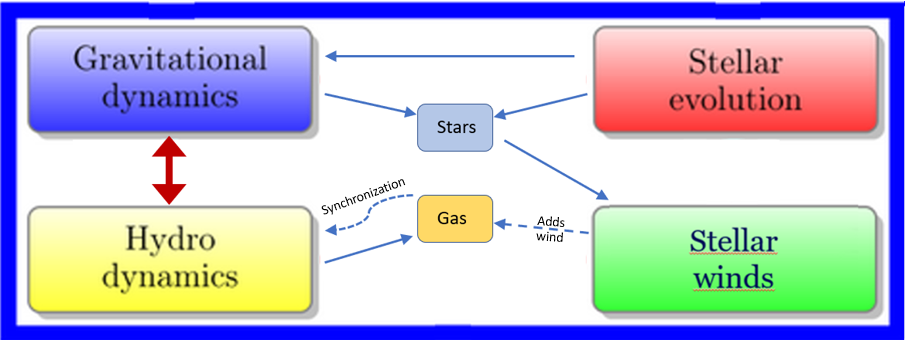
\includegraphics[width=0.8\textwidth]{figures/interactions.png}
    \caption{A diagram showing the different simulation codes and their interactions. The red arrow denotes a bridge between codes and the solid blue arrows show channels between codes.}
    \label{fig:m:interactions}
\end{figure*}

The second factor which can change the cluster stability over a longer duration of time is the effect of stellar winds.
During their lifetime, stars blow away a small part of their mass away in the form of gas.
The simulation for the stellar winds \parencite{stellar_wind.py} needs information on the evolutionary state of the stars, which is provided by the aforementioned SeBa-code.
The wind is created in the form of gas particles which are added to the the gas collection.


\subsection{Combining all codes}\label{sec:m:bridging}
For our project we used AMUSE for simulating stars and gas particles using hydrodynamics, gravitation, stellar evolution and stellar wind.
The codes also all have different timesteps, to find the right balance between the amount of detail and execution time of the simulation which are listed in Table \ref{tab:timesteps}.
The simulation runs for \SI{10}{\mega yr}.

\begin{table}[h]
    \centering
    \begin{tabular}{c|c}
        Code & Timestep (\si{\mega yr})\\
        \hline
        SPH \texttt{Fi} &  0.001\\
        N-body \texttt{ph4} & internal\\
        Stellar winds & 0.002\\
        Stellar evolution & 0.002\\
        Bridge & 0.002
    \end{tabular}
    \caption{The different timesteps used for each code. The smoothed particle hydrodynamics (SPH) code is used to simulate the evolution of the gas and the N-body code is used to simulate the gravitational effects between the stars. The N-body code timestep is not manually set, but it determines its timestep internally.}
    \label{tab:timesteps}
\end{table}


Since these different codes depend on the state of other codes, these states need to be communicated to each other.
To accomplish the communication between the codes we make use of bridges and channels, where a bridge is a two-way communication between codes and channel sends information in one direction.
The backbone of the simulation is the bridge between the hydrodynamics \texttt{Fi} code and gravitational \texttt{ph4} code as this simulates the actual interactions between interstellar medium and stars in the cluster.
The stellar evolution code is mostly independent of the other codes and primarily used to determine when a supernova takes place, because this will probably be one of the most impactful events on the amount of gas that is present in the cluster.
This is why we only need to channel the stellar evolution code to the stars of the cluster.
We have a channel from the stars to the code that simulates stellar winds, which tells this code where it should initialise its wind particles (at the stars) and how much wind it should create, based on the evolutionary state of the star.
The stellar winds code then generates new gas particles for the stellar wind and adds these to the existing gas collection.
Figure \ref{fig:m:interactions} shows a diagram visualising these interactions.


\section{Results}
\subsection{Initial simulations}
Our initial simulations did not give us the results we expected.
The stellar winds that were created did not seem to have an effect on the gas particles or bodies in the cluster.
At first we concluded that the wind particles were initialised too far outside of the cluster and as such did not have any interactions with the gas in the cluster.
We suspected that this was due to the high velocity of the particle (around 3000 km/s) in combination with too big timesteps (0.1 Myr).

\begin{figure}[b!]
    \centering
    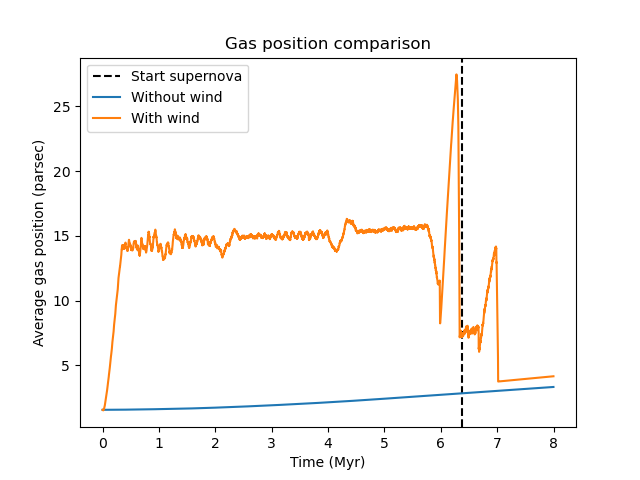
\includegraphics[width=0.9\linewidth]{figures/avg_pos3.png}
    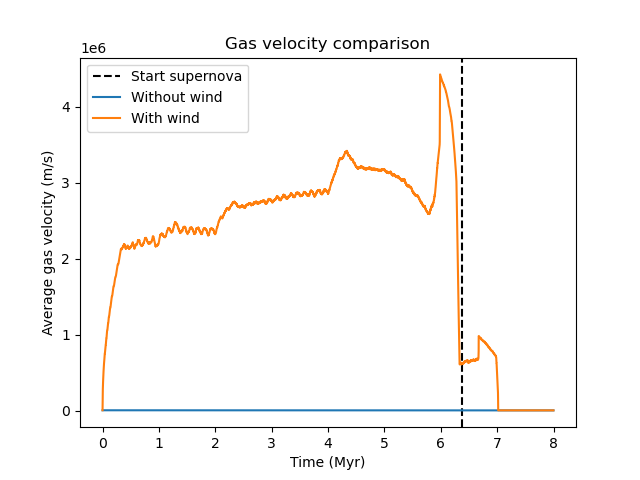
\includegraphics[width=0.9\linewidth]{figures/avg_vel3.png}
    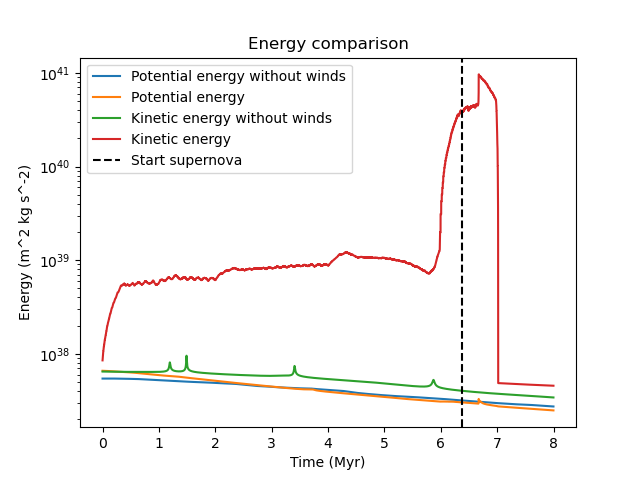
\includegraphics[width=0.9\linewidth]{figures/energy3.png}
    \caption{Results from a simulation of a cluster with and without stellar winds. The stellar wind particles are included in the gas.}
    \label{fig:r:Results3}
\end{figure}

\subsection{Simulations for the wind interaction problem}
From here on out we ran our simulations with 10 stars and 100 initial gas particles, so that the code would run faster and we would still be able to determine whether the interactions of the wind would be simulated or not.
One way we expected how this problem could be solved was by lowering the timesteps of most importantly the hydrodynamics code.
We calculated that we would need a timestep as small as \SI{60}{yr} to simulate the interactions of wind particles with the cluster every \SI{0.2}{pc}.
However, simulations with timesteps this small also failed to simulate the interactions, because wind particles were still initialised outside of the cluster. 


We tried to solve this problem by manually putting the initialised wind particles close to their origin star.
With this approach and the time step of the hydrodynamic code set to \SI{50}{yr} we ran a simulation with and without stellar wind and we examined the exact effect of the wind particles by plotting certain attributes of both simulations. We do this in order to visualise the precise effect that the stellar winds have on the cluster.
The three biggest attributes of interest were average distance from the centre of the gas, average velocity of the gas and kinetic and potential energy of the gas. The three attributes are plotted in Fig. \ref{fig:r:Results3} and for this simulation we used the timesteps in table \ref{tab:timesteps3}:
\begin{table}[]
    \centering
    \begin{tabular}{c|c}
         Code & dt (years) \\
         \hline
         Stellar evolution & 1000 \\
         Stellar winds & 2000 \\
         Bridge & 2000 \\
         Hydrodynamics & 1000 \\
    \end{tabular}
    \caption{Timesteps used for the simulation where we manually put wind particles near their origin.}
    \label{tab:timesteps3}
\end{table}

% 3:
        % self.dt = 0.001 | units.Myr
        % self.dt_winds = 0.0002 | units.Myr
        % self.dt_hydro = 0.0001 | units.Myr
        % self.dt_bridge = 0.0002 | units.Myr  #1.0*Pinner
        % self.supernovagasmass = (1|units.MSun)/10
        % self.windsgasmass = (1|units.MSun)/10000
        % self.n_stars = 10
        % self.n_gas = 100
        % self.r_cluster = 1.0 | units.parsec
        % self.t_end = 8 | units.Myr
        % self.settle_time = self.t_end - (8|units.Myr)

The average position plotted in Fig. \ref{fig:r:Results3} shows a small increase in distance compared to the simulation without stellar winds.
This is probably caused by the winds and the supernova, even though we would expect a much bigger effect.
The velocity seems to end at the same value, but this is because the difference between normal gas velocity and wind velocity is very big.
Figure \ref{fig:r:zoom-in} shows that there is in fact an increase in velocity of the normal gas of around 20\%.
Again, this is probably caused by the winds and supernova, but the effect is very small, compared to what we expected. 

\begin{figure}[h]
   \centering
   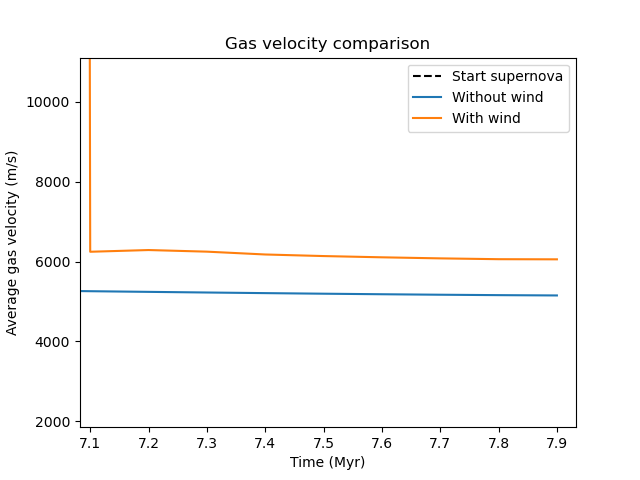
\includegraphics[width=0.9\linewidth]{figures/avg_vel3_endzoom.png}
   \caption{A zoom in on the tail of the second graph in Fig. \ref{fig:r:Results3} shows that there is a significant difference in velocity.}
   \label{fig:r:zoom-in}
\end{figure}

The average position has a plateau early in Fig. \ref{fig:r:Results3}.
This is the result of removing gas that left the system.
At roughly \SI{30}{pc} gas is removed and because wind is being created continuously, the average position of all the gas lies around \SI{15}{pc}.
There is a large drop off in both average position and velocity, but not in energy.
This is the result of our choice to make the wind particles of the supernova heavier than the normal stellar wind particles.
This means that less wind particles are created which means the average position and velocity are also lower (because the bulk of the gas collection is still in the cluster).
However the amount of energy that is created is not impacted by this choice, so this graph keeps its smooth curve.
A small time later the energy also has a drop off which is also present in the position and velocity graph, which happens because the wind particles from the supernova have reached the distance limit of \SI{30}{pc} and have been removed.


\subsection{Would-be result for our original cluster}
The small, but positive results (that show an increase in position, velocity and kinetic energy due to stellar winds) all come from our simulations with 10 stars and 100 gas particles.
So how does this relate to our initial open cluster?
The ratio between the number of stars and gas particles and their masses is the same, but we do not expect our results to hold for our initial cluster.
The energy needed to expel gas scales with both the gas and star mass, but the amount of wind that is created scales only slightly with star mass.
This is because the star that is the main cause of these stellar winds, the same star that goes supernova, has the same mass and mass loss in both clusters.
This means that the amount of energy turned into wind from this star does not increase.
So in the case of our initial cluster we expect the effect of the stellar wind and supernova on the density of the cluster to be relatively weaker. 



\section{Discussion}
\subsection{Flawed code}
The result we get is a lot smaller than the result that we expected.
Because experts told us that they normally get a larger effect, we suspect that the code still has some flaw. For example, while the code simulates some interactions correctly, it might not simulate every interaction that should be simulated or some connection between parts of the code could be missing.
AMUSE should be able to simulate all the interaction correctly and we know that it has been done before. However, even with tips from experts, we were not able to find the cause of our problem. We do know for certain that all the created wind particles are added to the hydrodynamics code. So as both the original gas particles and the wind particles are present in the hydrodynamics code, we would expect that all interactions between them would be simulated. 
On top of this we are certain that a timestep of \SI{50}{yr} for the hydrodynamics code is small enough to simulate the interactions. So the flaw must lie elsewhere.

Something that may point towards a flaw in the code is the fact that wind particles are still created some distance from their source (often outside of the cluster) and that we have to manually put them roughly at their origin. This correction should not be necessary if our code was flawless. However this correction worked well enough to allow us to find a small effect of the stellar winds on the cluster.

\subsection{Possible improvements}
The obvious improvement that can be made is fixing the flaws in the code. While we do not know where the flaws lie, we do know that they are present, because similar simulations have been run successfully in the past without the need for the corrections that we have used (like manually putting wind particles at their origin). Another way we could improve the code is by choosing a lower mass for the most massive star. This would result in lower velocities for the wind particles coming from that star allowing us to use bigger timesteps and this could possibly also reduce the initialisation distance from the parent star of the stellar wind particles. 
If the code works another improvement could be to separate the stellar wind simulation from the supernova simulation, so that you can use the best timesteps at the right time in both simulations and accurately deduce the ratios and masses of gas that is being blown away by either stellar winds or supernova as a sole cause.


\section{Conclusions}
The simulated effect of stellar winds and a supernova on the gas particles in an open cluster is a very small increase in separation and velocity of the gas particles.
However, because we expect a larger effect, we suspect that the code still has some flaws.
Due to the possible missing interactions between wind particles and gas particles in our simulation we were not able to conclusively deduce what effect stellar winds and supernovae have on the gas population in an open cluster.
We do suspect that the code is missing a small integral part that, when fixed, should allow the code to easily run the correct simulations, which might allow us to formulate an answer to our research question. 

\printbibliography

\end{document}

% Sources: 
% https://en.wikipedia.org/wiki/Open_cluster
% https://web.archive.org/web/20081222064251/http://seds.org/messier/open.html

% https://iopscience.iop.org/book/mono/978-0-7503-1320-9.pdf (boek van amuse)

% Mogelijk:
% Interessant boek? https://misaladino.com/wp-content/uploads/2019/11/Thesis_Martha_Irene.pdf

% https://academic.oup.com/mnras/article/476/4/5341/4923098
%   Measuring virial ratio of stars alone allows us to estimate how much mass a cluster will retain after gas expulsion to within 10 percent accuracy. (Regardles of structure of gas.
%   We conclude that gas removal may not be the main culprit for the dissolution of young star clusters.
%   Onderzoek erg vergelijkbaar met ons project!


% https://www.researchgate.net/figure/Distributions-of-gas-and-stars-in-the-early-phase-of-the-star-cluster-formation-t-426_fig1_48191381
%   (Misschien voor gasdistributie maar lijkt niet hoopvol)

% https://iopscience.iop.org/article/10.1088/0004-637X/778/2/118#references
%   AMUSE gebruikt voor N-body met collisions en stellar evolution
%   Misschien niet nuttig

% https://ui.adsabs.harvard.edu/abs/2013ApJ...774...10S/abstract
%   Velocity of gas pushed by supernova

% stellar winds.py:
% https://www.aanda.org/articles/aa/pdf/2019/05/aa32020-17.pdf